\chapter{awk}
\label{sec:awk}

如果要格式化报文或从一个大的文本文件中抽取数据包,那么awk可以完成这些任
务。它在文本浏览和数据的熟练使用上性能优异。与其它大多数Unix/Linux命令
不同的是,从名字上看,我们一眼看不出awk\index{awk}的功能:它既不是具有独立意义的英
文单词,也不是几个相关单词的缩写。事实上,awk是三个人名的缩写,他们是:
Aho、(Peter) Weinberg和(Brain)Kernighan。正是这三个家伙创造了awk,一个
优秀的样式扫描与处理工具。本章只介绍Gnu的awk版本gawk,其他awk版本不做介
绍。

awk的工作流程:
\begin{figure}[!h]
  \centering
  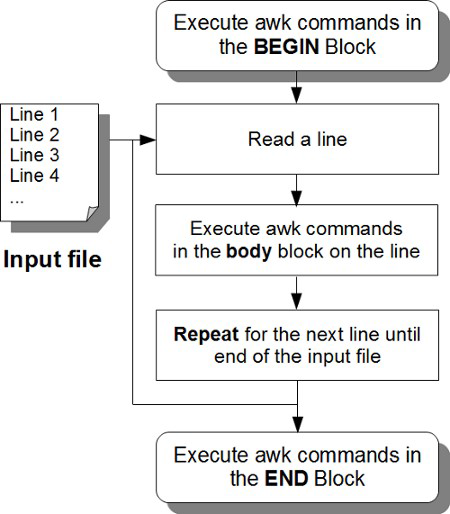
\includegraphics[width=.75\textwidth]{graph/awk_workflow.png}
  \caption{awk工作流程}
  \label{fig:awk_workflow}
\end{figure}

\section{初步使用}
\label{sec:FirstAwk}

假如我们有文件employee.txt,内容如下:

\small{
\begin{verbatim}
Beth	4.00	0
Dan	3.75	0
Kathy	4.00	10
Mark	5.00	20
Mary	6.50	22
Susie	6.25	18
\end{verbatim}
}
\normalsize

第一列表示员工姓名,第二列表示每小时加班所得的人民币,第三列为加班多少
小时。我们现在就来打印出那些加班大于0个小时的员工及其加班费,在命令行只
需执行这样一行命令即可:

\small{
\begin{verbatim}
awk '$3 > 0 { print $1, $2 * $3 }' employee.txt
\end{verbatim}
}
\normalsize

我们会得到这样的输出:

\small{
\begin{verbatim}
Kathy 40
Mark 100
Mary 143
Susie 112.5
\end{verbatim}
}
\normalsize

上面的命令告诉系统运行awk,使用单引号里的程序,并从employee.txt文件里获
得自己的数据。单引号里的部分完全就是awk程序。它包含了单个的
pattern-action(模式-动作)语句。动作\$3 >  0,匹配输入的每一行的第三列
或域,如果该列大于0,然后就执行下面的动作

\small{
\begin{verbatim}
{ print $1, $2 * $3 }
\end{verbatim}
}
\normalsize

对于每匹配到的行,就会打印第一个域并同时计算第二个域与第三个域的乘积。

如果我们想看看哪个家伙这个月没有加班,可以使用下面的命令:

\small{
\begin{verbatim}
awk '$3 == 0 { print $1 }' employee.txt
\end{verbatim}
}
\normalsize

这里的模式,\$3 == 0,将会匹配每一输入行的第三个域,如果等于0,就会执行下面的动作

\small{
\begin{verbatim}
{ print $1 }
\end{verbatim}
}
\normalsize

打印第一个域。

\section{awk程序结构}

awk的基本操作是对输入的行做逐一扫描,搜索这些行中匹配到的任意模式,然后
执行相应的动作。然后下一行被读进来并从头开始匹配到行末,直到输入文件的
所有行被读进来。就\$3 > 0来说,当满足时,说明该条件为真。

在上面的例子中,只有一个模式和动作,可以称为单pattern-action语句;对于
每一行,匹配到第三个字段等于0时,第一个字段将会被打印。

另外,模式和动作并不总是成对出现的,就是说,在pattern-action语句中,可
能只有模式或者只有动作。如果一个pattern没有相应的action,例如,

\small{
\begin{verbatim}
$3 == 0
\end{verbatim}
}
\normalsize

然后,每一被匹配的行都将会被打印,

\small{
\begin{verbatim}
Beth    4.00    0
Dan     3.75    0
\end{verbatim}
}
\normalsize

如果一个action没有pattern时,例如,

\small{
\begin{verbatim}
{ print $1 }
\end{verbatim}
}
\normalsize

此时,将会打印每一行的第一个域。由上可知,patterns和actions都是可选的。
actions使用大括号括起来以与patterns区分。

\subsection{BEGIN与END}

特殊的BEGIN模式在第一个输入文件的第一行被匹配,而END则是在最后一个文件的最后被处理后匹配。
下面的程序将会打印一个头部:

\small{
\begin{verbatim}
BEGIN { print "NAME     RATE    HOURS"; print "" }
      { print }
\end{verbatim}
}
\normalsize

我们将会得到这样的输出:

\small{
\begin{verbatim}
NAME     RATE   HOURS

Beth     4.00   0
Dan      3.75   0
Kathy    4.00   10
Mark     5.00   20
Mary     6.50   22
Susie    6.25   18
\end{verbatim}
}
\normalsize

我们可以在一行同时输入多条语句,这些语句之间需要用分号分开。注意到,\textit{print ""}意思是打印一个空行,
它与print不一样,仅仅一个print语句将打印整行。

\section{域和记录}
\label{sec:FieldRecordAwk}

awk执行时,其浏览域标记为\$1,\$2,...\$n。这种方法称为域标识。使用这些
域标识将更容易对域进一步处理。

\section{内置变量}

awk有一些内置的变量,变量如下:

\begin{table}[!h]
  \begin{center}
    \begin{tabular}{l|l}
      \hline
      变量     & 说明 \\
      \hline
      ARGC        & 命令行中参数的个数 \\
      \hline
      ARGV        & 包含命令行参数的数组 \\
      \hline
      CONVFMT     & 用于数字的字符串转换格式(默认格式为\%.6g) \\
      \hline
      ENVIRON     & 环境变量的关联数组 \\
      \hline
      FILENAME    & 当前文件名 \\
      \hline
      NR          & 当前记录的个数(当前的行号) \\
      \hline
      FNR         &  当前记录的个数(仅为当前文件,而非全部输入文件) \\
      \hline
      FS          & 字段分割符(默认为空格) \\
      \hline
      NF          & 当前记录中的字段个数 \\
      \hline 
      OFMT        & 数字的输出格式(默认格式为\%.6g) \\
      \hline
      OFS         & 输出字符的分割符(默认为空格) \\
      \hline
      ORS         & 输出记录分割符(默认为换行) \\
      \hline
    \end{tabular}
  \end{center}
\end{table}

\subsection{One-liners awk程序}

这一节介绍几个很有用的、短小精悍的awk程序。

\begin{enumerate}
\item 打印输入文件的总行数
\item 打印指定的行
\item 打印输入行的最后一个字段
\item 打印最后一行的最后一个字段
\item 打印每一输入行并擦除第二个字段
\end{enumerate}

\section{条件和循环}

这一节包含了一些基本的编程结构。它覆盖了awk程序设计语言中的所有控制结构。
在awk中,这些条件和循环的语法用起来比较简单。实际上,awk中的条件和循环
结构的语法借鉴C语言。因此,通过学习awk,我们也同样在学习C语言。

\subsection{if-else语句}

awk提供一个\textit{if-else}语句,这些语句只能用在actions中。下面的这个程序使用的还是\ref{sec:FirstAwk}节的例子。
在这个例子中,我们会计算那些每小时加班费大于6块的家伙,他们的总加班费及平均加班费。

\small{
\begin{verbatim}
# cat progfile
$2 > 6 { n = n + 1; pay = pay + $2 * $3 }
END    { if (n > 0)
            print n, "employees, total pay is", pay,
                     "average pay is", pay / n
         else
            print "no employees are paid more than Y6/hour"
}

# awk -f progfile employee.txt

\end{verbatim}
}
\normalsize

我们将会得到下面的输出结果:

\small{
\begin{verbatim}
  2 employees, total pay is 255.5 average pay is 127.75
\end{verbatim}
}
\normalsize

\subsection{while循环}
\label{subsec:WhileLoop}

while语句有一个condition和一个body。当condition为真时,body中的语句将被重复执行。我们使用下面的
程序计算这样的一个公式$ value = amount(1+rate)^{years} $

\small{
\begin{verbatim}
  # cat interest1 
  # interest1 - compute compound interest
  #   formula: value = amount(1+rate)^years
  #   input: amount rate years
  #   output: compounded value at the end of each year
  
  {  i = 1
    while (i <= $3) {
      printf("\t%.2f\n", $1 * (1 + $2) ^ i)
      i = i + 1
    }
  }
\end{verbatim}
}
\normalsize

如何执行该程序?看操作,

\small{
\begin{verbatim}
  # awk -f interest1 <- 回车
  1000 .06 5 <- 输入三组数字后,回车
  1060.00
  1123.60
  1191.02
  1262.48
  1338.23
\end{verbatim}
}
\normalsize

\subsection{for循环}
\label{subsec:ForLoop}

我们使用for语句改写第\ref{subsec:WhileLoop}节的while程序。如下:

\small{
\begin{verbatim}
  # cat interest2
  # interest2 - compute compound interest
  #   formula: value = amount(1+rate)^years
  #   input: amount rate years
  #   output: compounded value at the end of each year
  
  {  for (i = 1; i <= $3; i = i + 1)
    printf("\t%.2f\n", $1 * (1 + $2) ^ i)
  }
\end{verbatim}
}
\normalsize

\subsection{do循环}

\subsection{影响流控制的语句}

\section{数组}

数组是可以用来存储一组数据的变量。通常这些数据之间具有某种关系。数组中
的每一个元素通过它们在数组中的下标来访问。每个下标用方括号括起来。下面
的语句表示为数组中的一个元素赋值。

\begin{center}
\begin{verbatim}
  array[subscript] = value
\end{verbatim}
\end{center}


在awk中不必指明数组的大小,只需要为数组指定标示符。向数组元素赋值比较容
易。例如,下面的例子中为数组hr的一个元素指定了一个字符串“laven”。

\begin{verbatim}
  hr[1] = "laven"
\end{verbatim}

这个数组元素的下标是“1”,下面的语句将打印字符串“laven”。

\begin{verbatim}
  print hr[1]
\end{verbatim}

当然,我们可以用循环向数组中写入或取出元素。例如,如果数组hr有10个元素,
可以使用下面的循环来打印每个元素:

\begin{verbatim}
  hr_count = 10
  for (x = 1; x <= hr_count; ++x)
  print hr[x]
\end{verbatim}

我们来看一个例子,依然使用第\ref{sec:FirstAwk}节中的输入文件,让employee.txt文件反序输出,

\small{
\begin{verbatim}
  # cat reverse
  # reverse - print input in reverse order by line
  { line[NR] = $0 } # remember each input line
  END  { i = NR          # print lines in reverse order
    while (i > 0) {
      print line[i]
      i = i - 1
    }
  }
  
  # awk -f reverse employee.txt
  Susie    6.25   18
  Mary     6.50   22
  Mark     5.00   20
  Kathy    4.00   10
  Dan      3.75   0
  Beth     4.00   0
\end{verbatim}
}
\normalsize

\section{表达式}

\begin{verbatim}
[root@unionpay bash]# cat awk_file 
gold     1    1986  USA                 American Eagle
gold     1    1908  Austria-Hungary     Franz Josef 100 Korona
silver  10    1981  USA                 ingot
gold     1    1984  Switzerland         ingot
gold     1    1979  RSA                 Krugerrand
gold     0.5  1981  RSA                 Krugerrand
gold     0.1  1986  PRC                 Panda
silver   1    1986  USA                 Liberty dollar
gold     0.25 1986  USA                 Liberty 5-dollar piece
silver   0.5  1986  USA                 Liberty 50-cent piece
silver   1    1987  USA                 Constitution dollar
gold     0.25 1987  USA                 Constitution 5-dollar piece
gold     1    1988  Canada              Maple Leaf
\end{verbatim}

\begin{verbatim}
# This is an awk program that summarizes a coin collection.
#
/gold/    { num_gold++; wt_gold += $2 }      # Get weight of gold.
/silver/  { num_silver++; wt_silver += $2 }  # Get weight of silver.
END { val_gold = 485 * wt_gold;              # Compute value of gold.
    val_silver = 16 * wt_silver;           # Compute value of silver.
    total = val_gold + val_silver;
    print "Summary data for coin collection:";  # Print results.
    printf ("\n");
    printf ("   Gold pieces:                   %2d\n", num_gold);
    printf ("   Weight of gold pieces:         %5.2f\n", wt_gold);
    printf ("   Value of gold pieces:        %7.2f\n",val_gold);
    printf ("\n");
    printf ("   Silver pieces:                 %2d\n", num_silver);
    printf ("   Weight of silver pieces:       %5.2f\n", wt_silver);
    printf ("   Value of silver pieces:      %7.2f\n",val_silver);
    printf ("\n");
    printf ("   Total number of pieces:        %2d\n", NR);
    printf ("   Value of collection:         %7.2f\n", total);
}
\end{verbatim}

\begin{verbatim}
[root@unionpay bash]# awk -f myawk awk_file 
Summary data for coin collection:

   Gold pieces:                    9
   Weight of gold pieces:          6.10
   Value of gold pieces:        2958.50

   Silver pieces:                  4
   Weight of silver pieces:       12.50
   Value of silver pieces:       200.00

   Total number of pieces:        13
   Value of collection:         3158.50
\end{verbatim}

\section{函数}

\section{总结}
